\documentclass[aspectratio=169,10pt]{beamer}
\usepackage[utf8]{inputenc}
\usepackage[T1]{fontenc}
\usepackage{lmodern}
\usepackage[french]{babel}
\usepackage{booktabs}
\usepackage{tikz}
\usetikzlibrary{arrows.meta,positioning}
\graphicspath{{../figures/}{./}}

% Palette: sky/instrument tones of the 3D viewers.
\definecolor{ink}{HTML}{14212B}
\definecolor{muted}{HTML}{586A77}
\definecolor{sky}{HTML}{2F6DB0}
\definecolor{climb}{HTML}{17936A}
\definecolor{sink}{HTML}{C9502F}
\definecolor{therm}{HTML}{E39A2D}
\definecolor{paper}{HTML}{F6F8F9}
\setbeamercolor{normal text}{fg=ink,bg=paper}
\setbeamercolor{frametitle}{fg=ink,bg=paper}
\setbeamercolor{title}{fg=ink}
\setbeamercolor{structure}{fg=sky}
\setbeamercolor{alerted text}{fg=sink}
\setbeamerfont{frametitle}{series=\bfseries,size=\large}
\setbeamertemplate{navigation symbols}{}
\setbeamertemplate{itemize items}{\color{sky}\textbullet}
\setbeamertemplate{footline}{\hfill\color{muted}\scriptsize\insertframenumber\hspace{1em}\vspace{0.6em}}
\newcommand{\good}[1]{\textcolor{climb}{\textbf{#1}}}
\newcommand{\bad}[1]{\textcolor{sink}{\textbf{#1}}}
\newcommand{\fine}[1]{{\color{muted}\scriptsize #1}}

\title{GeneticWing}
\subtitle{Planifier le vol à voile d'un drone à voilure fixe :\\ professeur, élève génératif et recherche génétique dans un espace appris}
\author{Clément Dumeril}
\date{Bilan au 31 octobre 2026}

\begin{document}

\begin{frame}
  \titlepage
  \centering\fine{Toutes les valeurs viennent des runs du dépôt (README, Savio et PC de calcul). Coût : énergie nette dépensée, normalisée par le vol en palier au moteur ; $1$ = vol au moteur, $<0$ = énergie gagnée sur l'air.}
\end{frame}

% ---------------------------------------------------------------------------
\begin{frame}{En une page}
  \begin{itemize}
    \item \textbf{Problème.} Un planeur motorisé (SB-XC, 4{,}6\,m) doit gagner de l'énergie dans les thermiques au lieu de brûler sa batterie. Planifier ces trajectoires coûte cher (optimisation non convexe, contraintes de décrochage).
    \item \textbf{Ce qu'on a construit.} Un simulateur point-masse plat (+ aile par tronçons), un \emph{professeur} hors ligne (loi réactive + NLP), un jeu de 15\,080 situations résolues, un \emph{élève génératif} (VAE de commandes + simulateur), une recherche génétique dans son espace latent, une boucle fermée, et un vol longue distance de 20\,km.
    \item \textbf{Résultat central.} Le GA dans l'espace appris \good{bat son propre professeur} : $-5{,}72$ contre $-4{,}88$ (aile par tronçons, 65 situations de test), et la phase 3 sur point-masse donnait $-6{,}06$ contre $-5{,}24$.
    \item \textbf{En vol réel simulé.} En air calme, l'avance tient en boucle fermée ($-5{,}41$ contre $-4{,}69$). \bad{Une erreur de 15\,m sur le centre du thermique} fait tout retomber vers $-2$.
    \item \textbf{Sur 20\,km.} Les montées du GA sont \good{61\,\% plus rapides} (2{,}08 contre 1{,}29\,m/s) : $+3{,}3$\,km/h à batterie égale, ou \good{la vitesse du moteur avec 13 fois moins de batterie} ; \good{0 décrochage} grâce à un limiteur d'aile intérieure dans l'autopilote.
    \item \textbf{En temps réel.} Un générateur \emph{distillé} des solutions du GA, puis corrigé par DAgger sur les états du vol, \good{monte à 2{,}23\,m/s en 0{,}24\,s par plan} : aussi bien que le GA (13\,s), et plus vite que le moteur à MacCready 1.
  \end{itemize}
\end{frame}

% ---------------------------------------------------------------------------
\begin{frame}{Question de recherche et verdict des hypothèses}
  \small Un modèle génératif entraîné à imiter un optimiseur peut-il proposer vite des trajectoires de vol à voile proches de l'optimum, vérifiées par la physique et raffinées par l'optimisation locale ?\par\medskip
  \footnotesize
  \begin{tabular}{@{}p{0.27\linewidth}p{0.17\linewidth}p{0.48\linewidth}@{}}
    \toprule
    Hypothèse & Verdict & Ce qui le montre \\ \midrule
    H1 Le GA est un bon professeur & \bad{rejetée}, puis \good{reformulée} & GA sur 87 gènes : le plus faible à budget égal. Dans un espace latent appris : bat le professeur ($-0{,}82$). \\
    H2 Élève temps réel proche de l'optimum & \textbf{en partie} & Flow matching : 30--50\,ms, 67--90\,\% résolues, $\approx$40\,\% du gain. Prior physique : 0{,}2\,s, au niveau du professeur. \\
    H3 Multimodalité (régression échoue) & \good{tenue} & Régression : 0\,\% faisable (moyenne des deux sens d'orbite) ; flow matching : les deux sens. \\
    H4 Vérification + raffinement & \textbf{en partie} & NLP amorcée par l'élève : 76\,\% contre 8\,\% depuis le vol droit. \\
    H5 Robustesse (vent faux, rafales) & \textbf{ouverte} & Air calme : tient. Thermique mal placé : perte massive tant que la croyance n'est pas corrigée. \\
    H6 Auto-amélioration & \bad{non soutenue} & Une boucle d'amélioration : $-3{,}59 \to -3{,}73$, puis plus rien. \\
    \bottomrule
  \end{tabular}
\end{frame}

% ---------------------------------------------------------------------------
\begin{frame}{Le modèle physique}
  \begin{columns}[T]
    \column{0.52\linewidth}
    \small
    \begin{itemize}
      \item \textbf{Avion} : SB-XC, 4{,}2\,kg, 1{,}07\,m², allongement 19{,}8, polaire parabolique (finesse max 27, $V_{md}=8{,}05$\,m/s), moteur 15\,N. $C_{D0}$, $C_{L,\max}$, Oswald \emph{estimés}.
      \item \textbf{Point-masse en vol coordonné}, vent $W(p,t)$ : uniforme + thermique (échelle d'Allen, cœur gaussien de $\approx$30\,m de rayon à 250\,m) + turbulence de Dryden.
      \item \textbf{Platitude différentielle} : trajectoire + vent $\Rightarrow$ vitesse air, $C_L$, inclinaison, facteur de charge, poussée requise, sans intégration. Toute une population est évaluée d'un coup.
      \item \textbf{Aile par tronçons} (40 bandes) : en virage, l'aile intérieure vole plus lentement, ses sections décrochent avant l'aile moyenne, les ailerons saturent et traînent.
      \item \textbf{Intégration RK4} partout (voir la découverte Euler).
    \end{itemize}
    \column{0.45\linewidth}
    \centering
    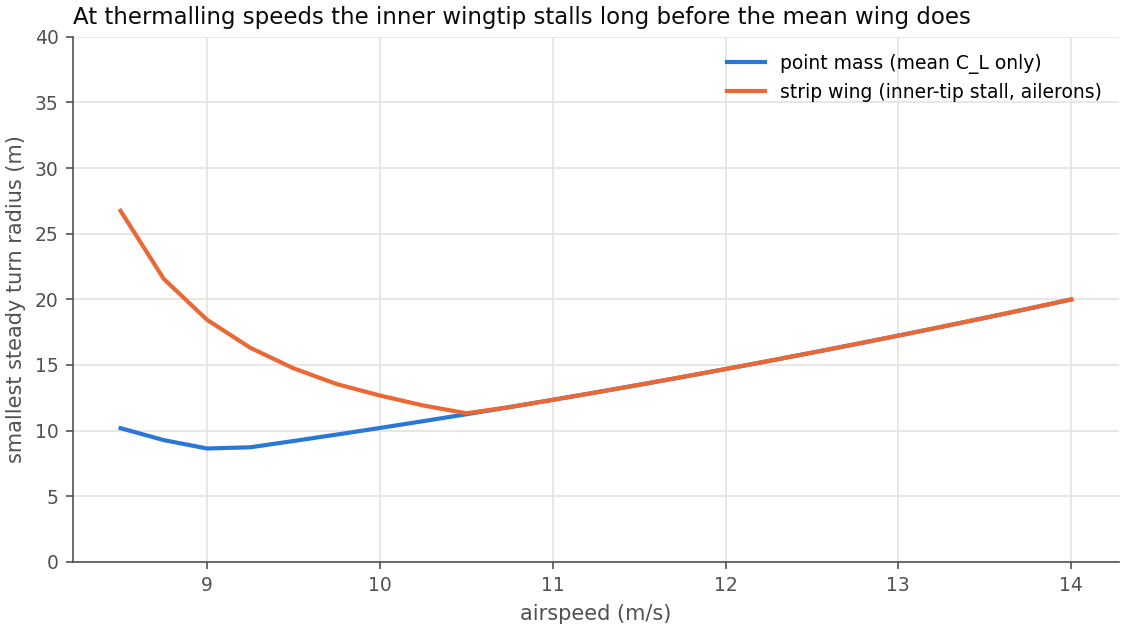
\includegraphics[width=\linewidth]{turn_limits.png}\\
    \fine{Rayon de virage minimal : 9\,m en point-masse à 9\,m/s, 18\,m avec l'aile par tronçons, $\approx$11\,m au mieux (10{,}5\,m/s).}
  \end{columns}
\end{frame}

% ---------------------------------------------------------------------------
\begin{frame}{L'architecture construite}
  \centering
  \begin{tikzpicture}[
      box/.style={draw=muted, rounded corners=3pt, fill=white, align=center, font=\scriptsize, minimum height=1.2cm, text width=2.2cm},
      main/.style={box, draw=climb, line width=1pt},
      arr/.style={-{Stealth[length=2mm]}, draw=muted, line width=0.7pt},
      lab/.style={font=\tiny, text=muted, align=center}]
    \node[box] (sim) {\textbf{Simulateur}\\plat + RK4\\aile par tronçons};
    \node[box, right=0.3cm of sim] (teach) {\textbf{Professeur}\\loi réactive (GA)\\+ NLP SLSQP, marges};
    \node[box, right=0.3cm of teach] (data) {\textbf{Données}\\15\,080 situations\\21\,034 trajectoires};
    \node[main, right=0.3cm of data] (vae) {\textbf{Élève génératif}\\VAE de commandes\\+ simulateur};
    \node[main, right=0.3cm of vae] (ga) {\textbf{GA latent}\\recherche dans\\l'espace appris};
    \node[box, below=1.1cm of ga] (cl) {\textbf{Boucle fermée}\\autopilote, rafales,\\croyance fausse, MPC};
    \node[box, left=0.3cm of cl] (xc) {\textbf{20\,km}\\tacticien MacCready\\+ montées planifiées};
    \node[box, left=0.3cm of xc] (lim) {\textbf{Sécurité}\\limiteur d'aile\\intérieure};
    \draw[arr] (sim) -- (teach); \draw[arr] (teach) -- (data); \draw[arr] (data) -- (vae); \draw[arr] (vae) -- (ga);
    \draw[arr] (ga) -- (cl); \draw[arr] (cl) -- (xc); \draw[arr] (lim) -- (xc);
    \node[lab, above=0.05cm of teach] {phase 2};
    \node[lab, above=0.05cm of data] {Savio};
    \node[lab, above=0.05cm of vae] {phase 3};
    \node[lab, below=0.05cm of cl] {phase 4};
    \node[lab, below=0.05cm of xc] {phase 5};
  \end{tikzpicture}\par\medskip
  \small Le professeur coûte $\approx$35\,s par situation ; on l'amortit une fois hors ligne. L'élève propose des plans en 0{,}2\,s (prior) à 13\,s (GA, 3\,000 évaluations). Chaque plan est vérifié par le simulateur.
\end{frame}

% ---------------------------------------------------------------------------
\begin{frame}{Les algorithmes d'optimisation utilisés}
  \footnotesize
  \begin{tabular}{@{}p{0.25\linewidth}p{0.42\linewidth}p{0.27\linewidth}@{}}
    \toprule
    Algorithme & Rôle et détails & Où \\ \midrule
    GA à codage réel & croisement SBX, mutation polynomiale, classement de Deb (faisable d'abord, puis violation), population 50 réglée par balayage & phase 2, GA latent \\
    GA de T. Zohdi & 80\,\% d'immigrants aléatoires par génération ; règle les 10 paramètres de la loi réactive & loi réactive \\
    CMA-ES & stratégie d'évolution à covariance adaptative, référence & phase 2 \\
    NLP SLSQP & optimisation locale sous contraintes, gradients par différences finies vectorisées, budget strict, multi-départ & professeur, raffinement \\
    Loi réactive d'orbite & guidage par cap + énergie (rayon, vitesses, centre, plancher) ; 2 graines par sens d'orbite (normale et rapide) & graines du professeur \\
    Contraintes & agrégation KS, marges du professeur (\emph{constraint tightening} : $C_L$ 0{,}75, inclinaison 38°, charge 2{,}1, poussée 0{,}8) & partout \\
    MPC & replanification toutes les 10\,s, horizon qui rétrécit jusqu'à la fin du vol, démarrage à chaud & phase 4 \\
    Théorie de MacCready & vitesse de transition optimale, choix du thermique au meilleur rythme de progression, sortie sous le réglage & phase 5 \\
    \bottomrule
  \end{tabular}
\end{frame}

% ---------------------------------------------------------------------------
\begin{frame}{Les modèles de machine learning utilisés}
  \footnotesize
  \begin{tabular}{@{}p{0.26\linewidth}p{0.45\linewidth}p{0.23\linewidth}@{}}
    \toprule
    Modèle & Ce qu'il apprend & Résultat \\ \midrule
    Régression MLP (4$\times$512) & contexte $\to$ génome, déterministe & \bad{0\,\%} faisable \\
    Flow matching conditionnel (rectified flow) & distribution des trajectoires du professeur ; 1 ou 8 pas d'échantillonnage & 67--90\,\% résolues, 30--50\,ms \\
    VAE conditionnel de positions & compresse les 87 gènes en $d=8/16/32$ dimensions latentes & GA latent : 100\,\% résolues, $-3{,}59$ \\
    \textbf{VAE de commandes + décodeur physique} & sort $C_L$, inclinaison, poussée en 61 n\oe uds, bornés par construction ; un simulateur RK4 différentiable (PyTorch) en fait la trajectoire & \good{faisabilité 20\,\% $\to$ 100\,\%} \\
    Évolution de variables latentes & le GA cherche dans l'espace latent, chaque individu est décodé et volé (Volz et al.~2018) & \good{bat le professeur} \\
    Données & contexte dans le repère de cap (invariance par rotation), miroir gauche/droite exact, marges du professeur & \\
    \bottomrule
  \end{tabular}\par\medskip
  \fine{Entraînement : CPU (PC) et GPU A40 (Savio) ; 20\,000 pas ; $\beta$-VAE avec $\beta=0{,}1$ ; décodeur 3$\times$512.}
\end{frame}

% ---------------------------------------------------------------------------
\begin{frame}{Phase 1 : socle, reproduction du plané de l'ARPL (S0)}
  \centering\small
  \begin{tabular}{@{}lccc@{}}
    \toprule
    Mesure & Vol ARPL & Plan, vent uniforme & Boucle fermée, Dryden (50 tirages) \\ \midrule
    Vitesse air moyenne (m/s) & 12{,}50 & 12{,}50 & 12{,}61 \\
    Taux de chute moyen (m/s) & 1{,}48 & 1{,}58 & 1{,}61 \\
    Finesse & 9{,}83 & 11{,}15 & 11{,}27 \\
    RMSE vitesse air (m/s) & 1{,}09 & 0{,}00 & 0{,}87 \\
    RMSE netto (m/s) & 0{,}69 & 0{,}00 & 0{,}71 \\
    \bottomrule
  \end{tabular}\par\medskip
  \begin{itemize}\small
    \item Les statistiques d'erreur du vol réel de l'ARPL sont retrouvées en boucle fermée ; le planificateur converge depuis 20 départs perturbés sur 20.
    \item La contrainte $T_{req}=0$ généralise la contrainte de taux de chute de l'ARPL à un vent non uniforme.
  \end{itemize}
  \fine{Masse et surface du Stratosurfer : valeurs provisoires ; finesse simulée au-dessus du vol réel (pas de pertes de suivi hors turbulence).}
\end{frame}

% ---------------------------------------------------------------------------
\begin{frame}{Phase 2 : quel professeur ? (3 scénarios $\times$ 3 instances $\times$ 11 méthodes)}
  \begin{columns}[T]
    \column{0.53\linewidth}
    \scriptsize
    \begin{tabular}{@{}lccc@{}}
      \toprule
      Méthode (20k éval.) & S1 thermique & S2 vers but & S3 pente \\ \midrule
      NLP (départ droit) & $-2{,}77$ & infais. & $-2{,}11$ \\
      GA réglé (pop.~50) & $0{,}15$ & infais. & $-0{,}73$ \\
      GA de Zohdi & infais. & infais. & infais. \\
      CMA-ES + NLP & $-3{,}80$ & infais. & \good{$-2{,}16$} \\
      GA @100k & $-0{,}99$ & $0{,}47$ & $-1{,}83$ \\
      Loi réactive & $-4{,}58$ & \good{$-0{,}02$} & $-1{,}96$ \\
      \textbf{Loi + NLP} & \good{$-6{,}04$} & infais. & $-0{,}03$ \\
      \bottomrule
    \end{tabular}\par\medskip
    \small
    \begin{itemize}
      \item \bad{H1 rejetée telle quelle} : le GA brut est le plus faible à budget égal (87 à 159 gènes couplés).
      \item \good{La structure bat la recherche} : la loi réactive encode l'orbite ; ajustée puis raffinée par la NLP, elle donne le meilleur professeur ($+30$\,\% d'énergie sur la loi seule).
    \end{itemize}
    \column{0.45\linewidth}
    \centering
    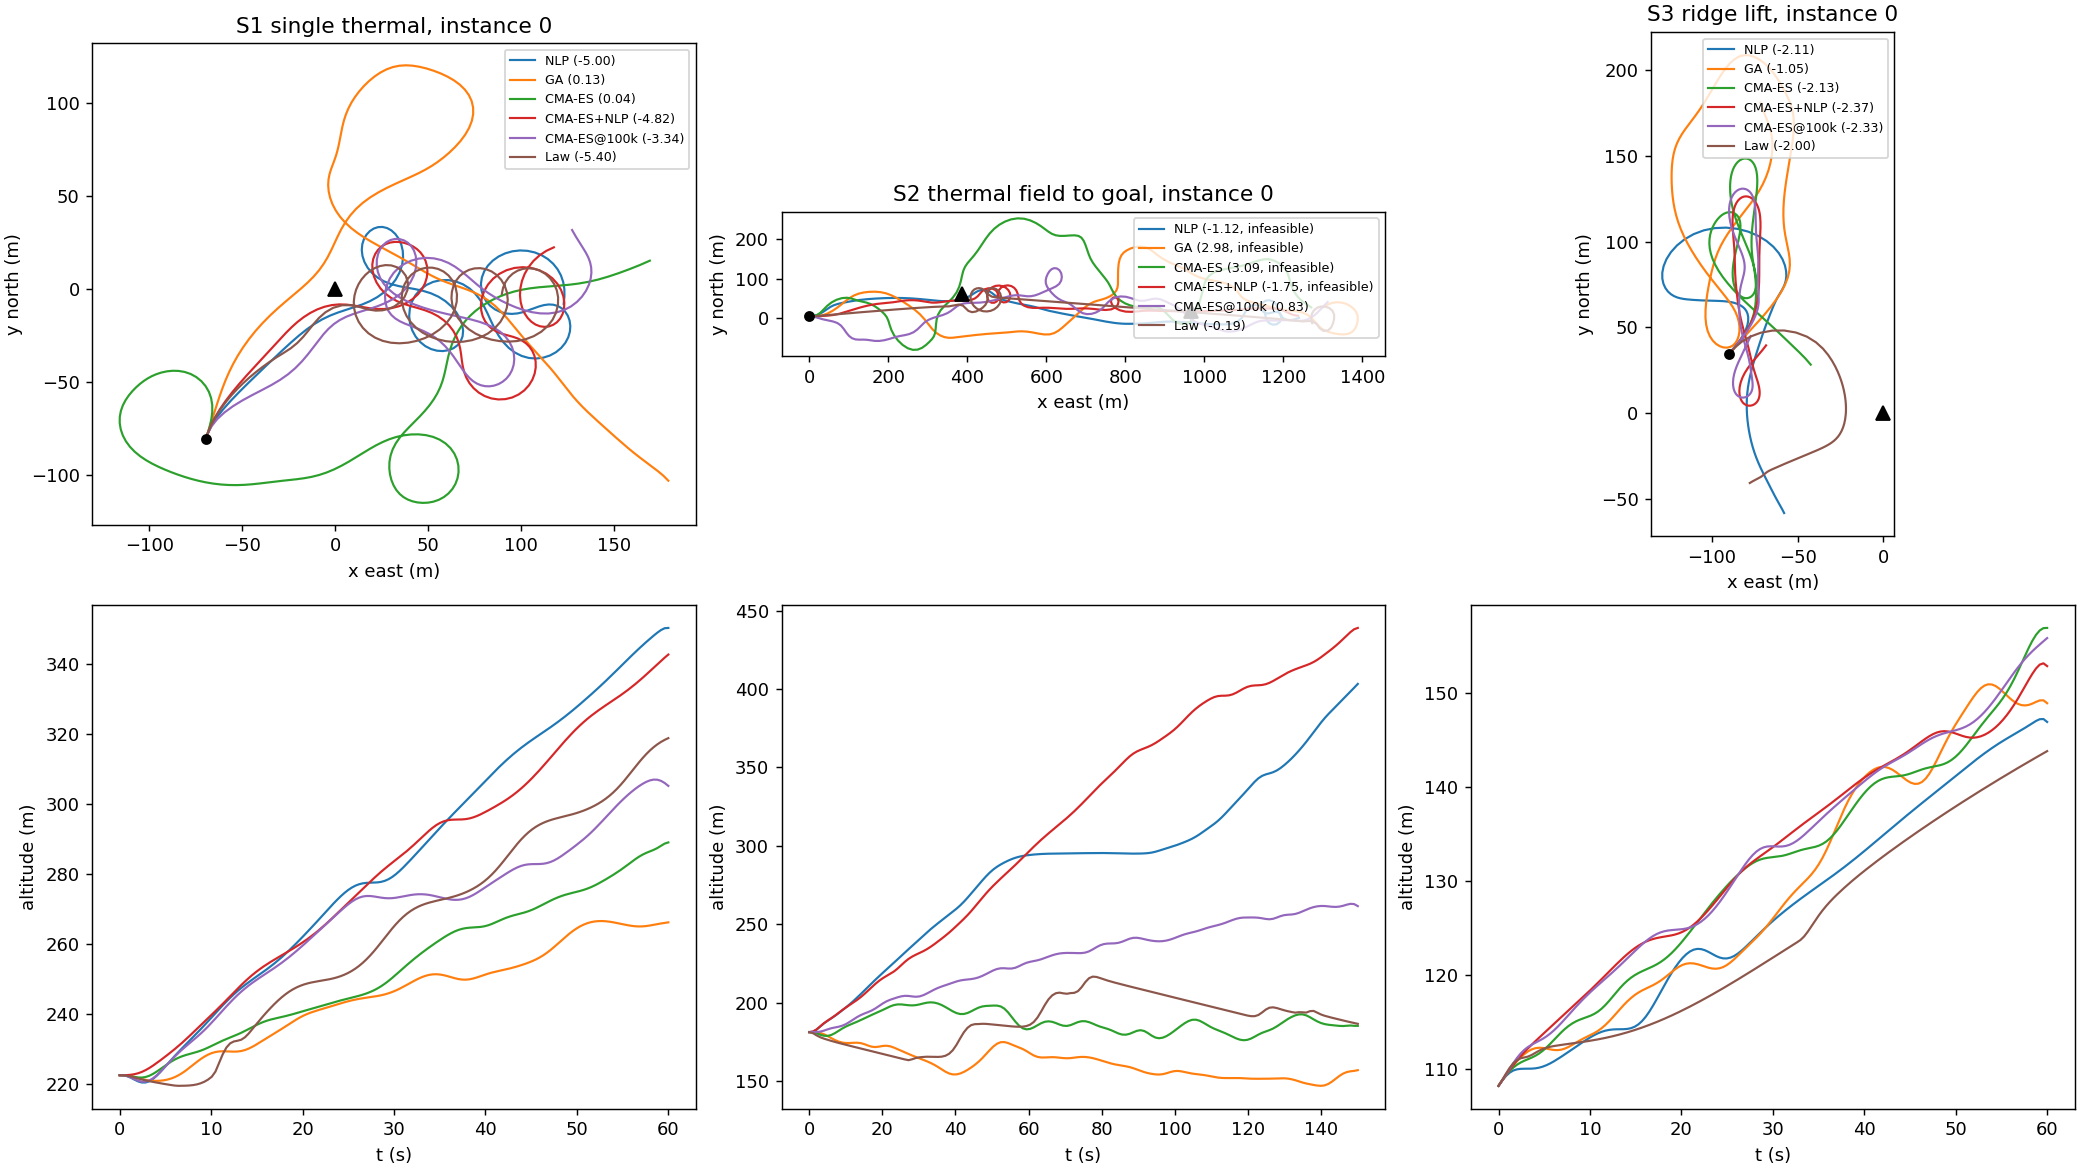
\includegraphics[width=\linewidth]{phase2_trajectories.png}
  \end{columns}
\end{frame}

% ---------------------------------------------------------------------------
\begin{frame}{Phase 3a : élève génératif (78 situations nouvelles, professeur $-5{,}19$)}
  \begin{columns}[T]
    \column{0.6\linewidth}
    \scriptsize
    \begin{tabular}{@{}lcccc@{}}
      \toprule
      Méthode & Résolues & Coût & Écart & Temps \\ \midrule
      Régression & \bad{0\,\%} & -- & -- & 1\,ms \\
      Flow matching, 64 tirages, 1 pas & 90\,\% & $0{,}87$ & $6{,}11$ & 28\,ms \\
      Flow matching, 8 pas & 67\,\% & $-2{,}06$ & $3{,}11$ & 49\,ms \\
      + mutations + NLP & 76\,\% & $-2{,}51$ & $2{,}72$ & 1{,}0\,s \\
      Loi réactive & 100\,\% & $-3{,}53$ & $1{,}66$ & réflexe \\
      NLP depuis vol droit & 8\,\% & $1{,}49$ & $6{,}95$ & 0{,}9\,s \\
      \bottomrule
    \end{tabular}
    \column{0.38\linewidth}
    \small
    \begin{itemize}
      \item \good{H3} : la régression moyenne l'orbite horaire et anti-horaire en une ligne droite qui sort du thermique.
      \item \textbf{La faisabilité est le goulot} : un professeur résolu pile sur ses contraintes cassait 80\,\% de ses solutions au moindre bruit ; avec des marges ($-0{,}24$ d'énergie), 8 à 16 fois plus tolérant.
    \end{itemize}
  \end{columns}\par\smallskip
  \centering
  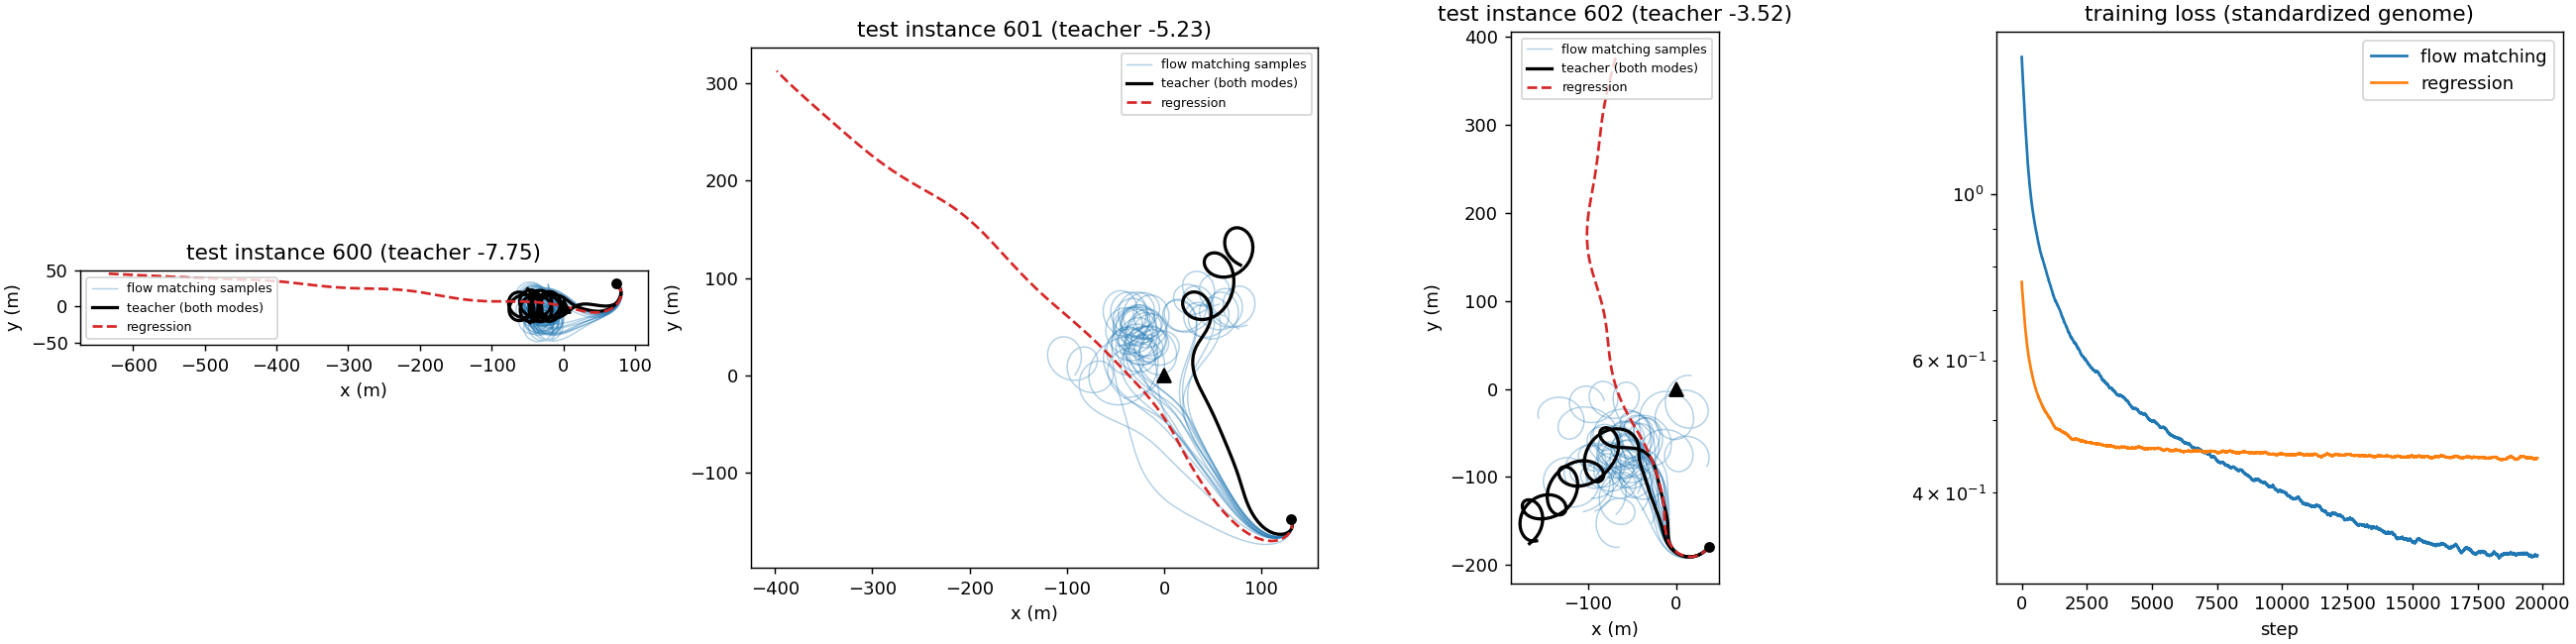
\includegraphics[width=0.92\linewidth,height=0.33\textheight,keepaspectratio]{phase3_student.png}
\end{frame}

% ---------------------------------------------------------------------------
\begin{frame}{Phase 3b : à l'échelle (Savio, 15\,080 situations)}
  \begin{columns}[T]
    \column{0.5\linewidth}
    \centering
    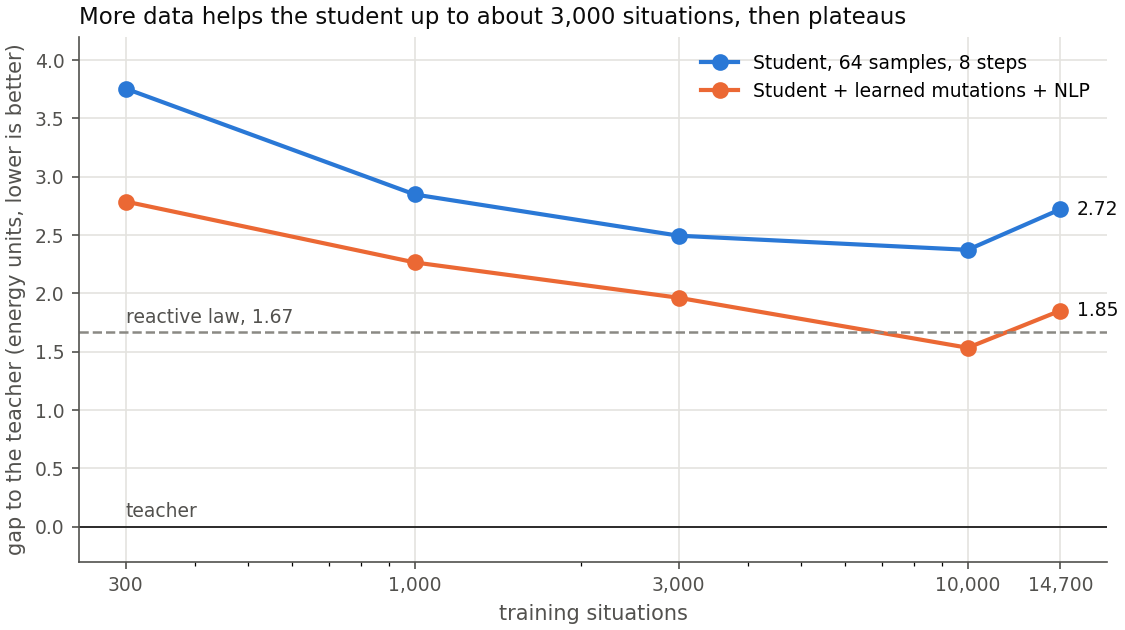
\includegraphics[width=\linewidth]{savio_scaling.png}
    \column{0.48\linewidth}
    \small
    \begin{itemize}
      \item Le professeur résout 15\,080 situations (27\,649 solutions) sur 21 n\oe uds de 32 c\oe urs.
      \item \textbf{Courbe d'échelle} : plus de données aide jusqu'à $\approx$3\,000 situations, puis l'écart plafonne. Au-delà, la limite est le modèle, pas les données.
      \item H3 tient à toutes les tailles : la régression résout au plus 12\,\%.
      \item Sur les 77 situations de test Savio : professeur $-5{,}24$, loi réactive $-3{,}57$, flow matching + NLP $-3{,}54$.
    \end{itemize}
  \end{columns}
\end{frame}

% ---------------------------------------------------------------------------
\begin{frame}{Phase 3c : GA dans un espace appris (77 situations, professeur $-5{,}24$)}
  \begin{columns}[T]
    \column{0.57\linewidth}
    \scriptsize
    \begin{tabular}{@{}lccc@{}}
      \toprule
      Méthode & Résolues & Coût & Écart \\ \midrule
      GA sur 87 gènes + NLP & 55\,\% & $+1{,}92$ & $7{,}09$ \\
      GA latent (VAE de positions) + NLP & 100\,\% & $-3{,}59$ & $1{,}64$ \\
      Commandes du professeur, volées & 100\,\% & $-4{,}70$ & $0{,}54$ \\
      \textbf{64 tirages du prior physique} & 100\,\% & \good{$-5{,}21$} & \good{$0{,}03$} \\
      \textbf{GA latent, décodeur physique} & 100\,\% & \good{$-6{,}06$} & \good{$-0{,}82$} \\
      \bottomrule
    \end{tabular}\par\medskip
    \small
    \begin{itemize}
      \item L'espace latent \good{sauve le GA} : 55\,\% $\to$ 100\,\% résolues.
      \item Mettre \textbf{la physique dans le décodeur} (commandes bornées + simulateur) fait passer l'aller-retour de 20\,\% à 100\,\% faisable.
      \item 64 tirages, sans recherche, \good{égalent le professeur en 0{,}2\,s}.
    \end{itemize}
    \column{0.41\linewidth}
    \centering
    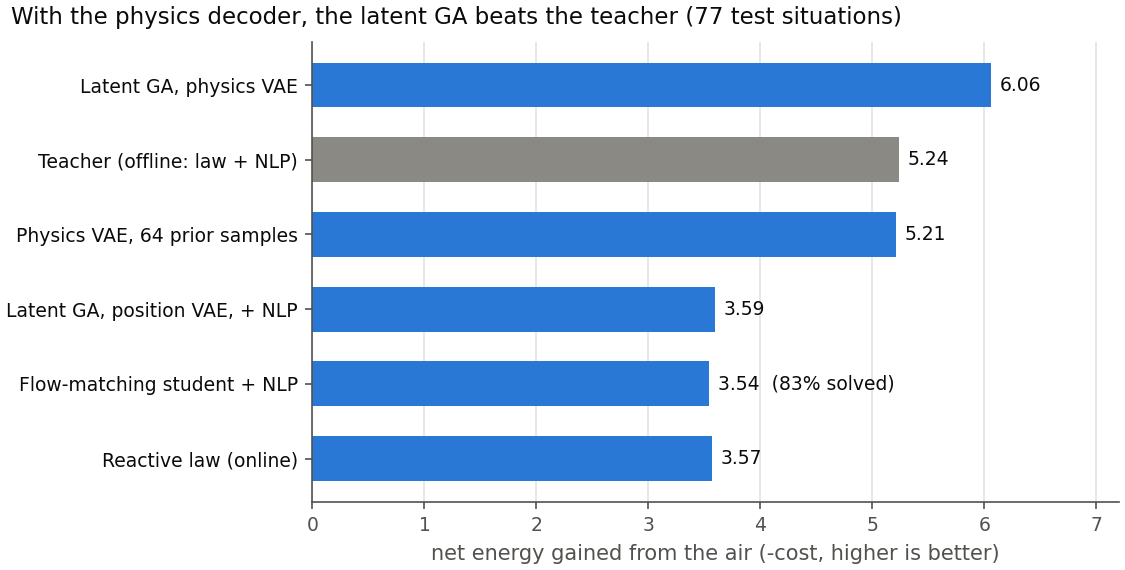
\includegraphics[width=\linewidth]{savio_methods.png}
  \end{columns}
\end{frame}

% ---------------------------------------------------------------------------
\begin{frame}{Une découverte méthodologique : la recherche exploite l'erreur numérique}
  \begin{columns}[T]
    \column{0.55\linewidth}
    \small
    \begin{itemize}
      \item Les premiers simulateurs intégraient en \textbf{Euler explicite}. En virage, la portance fait tourner la vitesse, et chaque pas ajoute $(a\,\Delta t)^2$ à son carré : \bad{de l'énergie gratuite}.
      \item Le GA sur le décodeur physique l'a trouvée et exploitée : des coûts \bad{trois fois meilleurs que le professeur}, physiquement impossibles.
      \item Correction : \textbf{RK4 partout}. Un virage stabilisé perd exactement le taux de chute de la polaire, même à pas de 0{,}4\,s.
      \item Seule la loi réactive était touchée en ligne : $-3{,}73$ (Euler) contre $-3{,}57$ (RK4).
    \end{itemize}
    \column{0.42\linewidth}
    \begin{block}{Leçon}
      \small Un optimiseur puissant branché sur un simulateur trouve ses défauts avant de trouver la physique. Tout gain surprenant doit être vérifié par un intégrateur plus précis.
    \end{block}
  \end{columns}
\end{frame}

% ---------------------------------------------------------------------------
\begin{frame}{Réalisme : l'avance venait-elle de virages impossibles ?}
  \begin{columns}[T]
    \column{0.48\linewidth}
    \scriptsize
    \textbf{Un même rayon minimal pour tous} (77 situations)\par\smallskip
    \begin{tabular}{@{}lccc@{}}
      \toprule
      Rayon min. & Professeur & GA latent & Écart \\ \midrule
      aucun & $-5{,}22$ & $-6{,}06$ & \good{$-0{,}85$} \\
      12\,m & $-5{,}22$ & $-5{,}86$ & \good{$-0{,}64$} \\
      15\,m & $-5{,}23$ & $-5{,}56$ & \good{$-0{,}35$} \\
      18\,m & $-5{,}09$ & $-4{,}42$ & \bad{$+0{,}67$} \\
      \bottomrule
    \end{tabular}\par\medskip
    \textbf{Aile par tronçons, VAE entraîné en point-masse}\par\smallskip
    \begin{tabular}{@{}lcc@{}}
      \toprule
      Méthode & Résolues & Coût \\ \midrule
      Professeur & 100\,\% & $-4{,}70$ \\
      GA latent & 100\,\% & \bad{$-4{,}28$} \\
      64 tirages du prior & 66\,\% & $-1{,}23$ \\
      \bottomrule
    \end{tabular}
    \column{0.5\linewidth}
    \small
    \begin{itemize}
      \item Le GA gagnait surtout \textbf{en serrant ses cercles} (rayon médian 15--25\,m contre 21--29\,m).
      \item Avec la vraie limite physique (décrochage de l'aile intérieure), \bad{l'avance disparaît} : l'espace latent appris en point-masse ne contient pas les bons cercles.
      \item \textbf{Correction dans les données} : régénérer le professeur avec l'aile par tronçons et réentraîner (page suivante).
    \end{itemize}
  \end{columns}
\end{frame}

% ---------------------------------------------------------------------------
\begin{frame}{Aile par tronçons : professeur corrigé et réentraînement}
  \begin{columns}[T]
    \column{0.5\linewidth}
    \small
    \textbf{Pourquoi le professeur échouait sur 39\,\% des situations} (128 analysées) : dans 100\,\% des cas, la NLP finit avec \textbf{l'aile intérieure décrochée}.\par\smallskip
    \scriptsize
    \begin{tabular}{@{}lcc@{}}
      \toprule
      Graine de la NLP & Faisable & Coût \\ \midrule
      \textbf{Orbite plus rapide} & \good{52\,\%} & $-4{,}63$ \\
      Plané droit & 40\,\% & $+0{,}91$ \\
      Orbite plus large (80--120\,m) & 9--19\,\% & $\approx+1$ \\
      Sans marges & 23--33\,\% & $\approx-5{,}3$ \\
      \bottomrule
    \end{tabular}\par\medskip
    \small Une orbite \emph{plus rapide} (pas plus large) baisse le $C_L$ et rend une marge à l'aile intérieure. Professeur à 2 graines : \good{39\,\% $\to$ 17\,\%} non résolues ; l'orbite rapide gagne 83\,\% des trajectoires.
    \column{0.48\linewidth}
    \scriptsize
    \textbf{Réentraîné, Savio, 15\,080 situations, 65 tests}\par\smallskip
    \begin{tabular}{@{}lccc@{}}
      \toprule
      Méthode & $d=8$ & $d=16$ & $d=32$ \\ \midrule
      Professeur & $-4{,}88$ & $-4{,}88$ & $-4{,}88$ \\
      Commandes du prof., volées & $-4{,}45$ & $-4{,}45$ & $-4{,}45$ \\
      64 tirages du prior & $-4{,}72$ & $-4{,}64$ & $-4{,}65$ \\
      \textbf{GA latent} & $-5{,}37$ & $-5{,}69$ & \good{$-5{,}72$} \\
      \bottomrule
    \end{tabular}\par\medskip
    \small \good{L'avance revient : $-0{,}84$}, la même que pour le point-masse ($-0{,}82$). Le prior repasse de 66\,\% à 100\,\% résolues.\par
    \fine{Piège rencontré : la loi réglée \emph{sous} l'aile par tronçons convergeait vers des orbites irréparables (3/16 faisables contre 13/16) ; elle est réglée en point-masse et ne sert que de graine.}
  \end{columns}
\end{frame}

% ---------------------------------------------------------------------------
\begin{frame}{Sensibilité à la polaire estimée du SB-XC (65 situations, $d=16$)}
  \begin{columns}[T]
    \column{0.55\linewidth}
    \scriptsize
    \begin{tabular}{@{}lcccc@{}}
      \toprule
      Avion & Professeur (résolues) & Prior & GA latent & Écart \\ \midrule
      nominal & $-4{,}91$ (100\,\%) & $-4{,}64$ & $-5{,}69$ & \good{$-0{,}79$} \\
      $C_{D0}\times0{,}8$ & $-5{,}48$ (100\,\%) & $-5{,}13$ & $-6{,}29$ & $-0{,}81$ \\
      $C_{D0}\times1{,}2$ & $-4{,}44$ (100\,\%) & $-4{,}24$ & $-5{,}23$ & $-0{,}79$ \\
      $C_{L,\max}\times1{,}2$ & $-5{,}30$ (100\,\%) & $-5{,}29$ & $-6{,}24$ & $-0{,}94$ \\
      masse $\times0{,}8$ & $-5{,}70$ (100\,\%) & $-5{,}57$ & $-6{,}93$ & $-1{,}23$ \\
      $C_{L,\max}\times0{,}8$ & $-4{,}11$ (89\,\%) & $-2{,}53$ & $-4{,}49$ & \bad{$-0{,}09$} \\
      masse $\times1{,}2$ & $-4{,}36$ (100\,\%) & $-2{,}81$ & $-4{,}49$ & \bad{$-0{,}13$} \\
      \bottomrule
    \end{tabular}
    \column{0.42\linewidth}
    \small
    \begin{itemize}
      \item \textbf{La traînée ne compte pas} pour la comparaison : tout bouge de $\approx$0{,}5, l'écart reste à $-0{,}8$.
      \item \textbf{La marge au décrochage gouverne} : avion plus lourd ou $C_{L,\max}$ plus faible $\Rightarrow$ l'avance tombe à $-0{,}1$ (toujours positive).
      \item Sans recherche, le prior \bad{ne se transfère pas} à un autre avion.
      \item À mesurer sur l'avion réel : \textbf{charge alaire et $C_{L,\max}$}.
    \end{itemize}
  \end{columns}
\end{frame}

% ---------------------------------------------------------------------------
\begin{frame}{Phase 4 : boucle fermée, ce que l'avion vole vraiment}
  \centering
  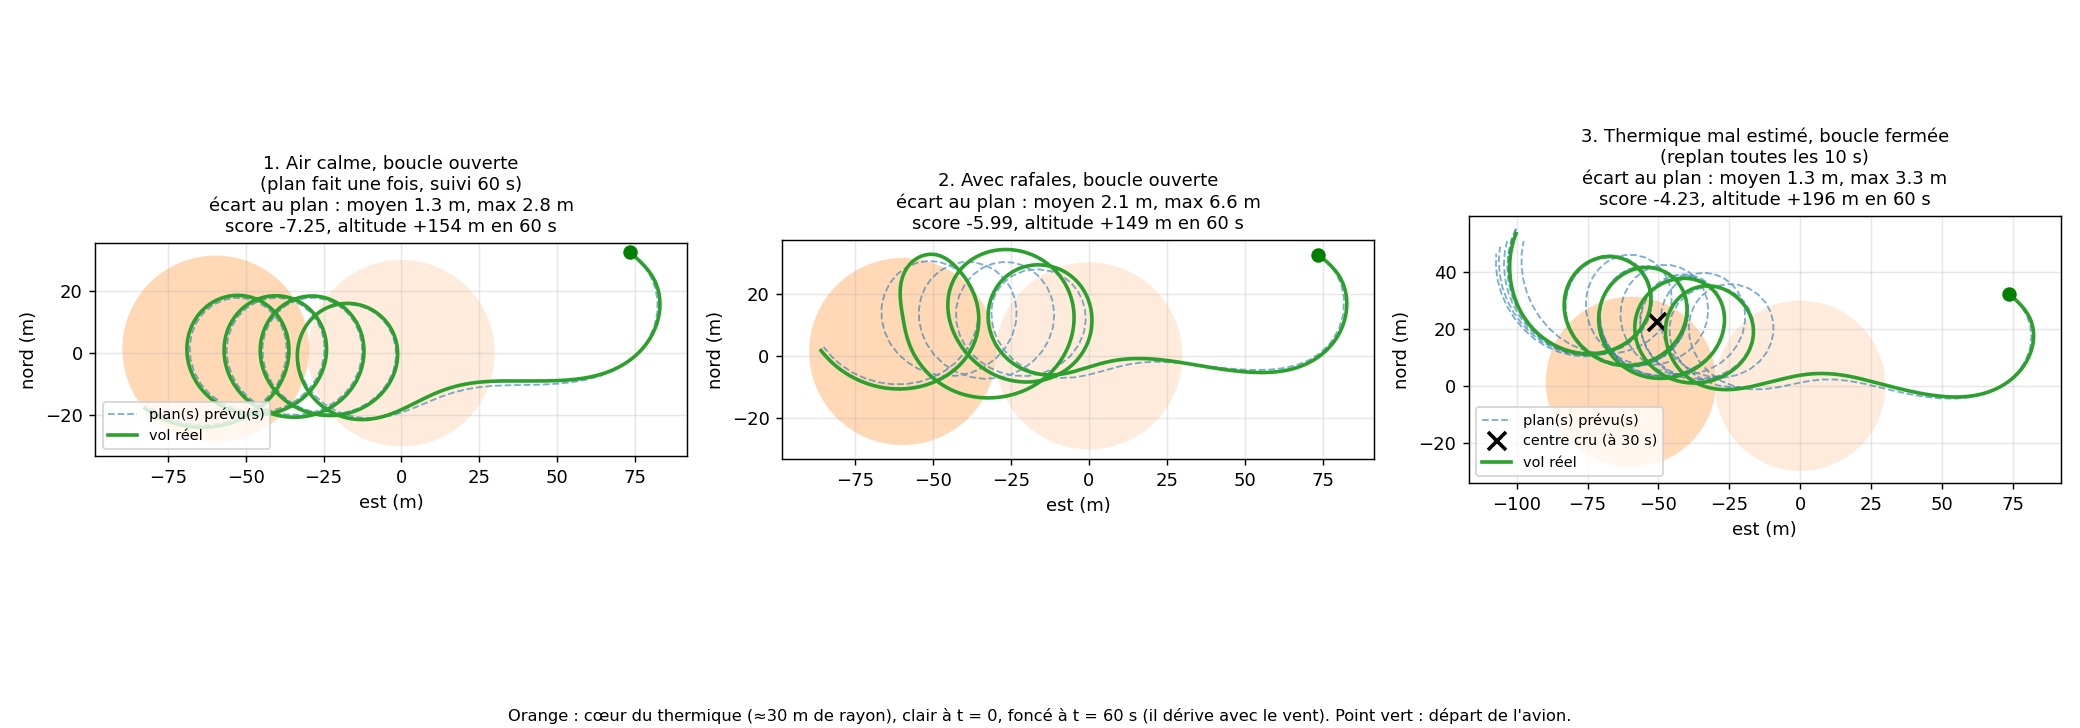
\includegraphics[width=0.94\linewidth]{closed_loop_tracking.png}\par
  \small L'autopilote suit le plan à \textbf{1--2\,m en moyenne} (6{,}6\,m au pire en rafales). Avec un centre de thermique faux de $\approx$15\,m, la spirale est propre mais \bad{décalée} : l'avion monte en brûlant 4 fois plus de batterie.\par
  \fine{Autopilote : retard d'attitude 0{,}3\,s, roulis limité, protection $C_L$ à 90\,\%, inclinaison $\le$40°, traînée d'aileron. MPC : replan toutes les 10\,s, horizon jusqu'à la fin du vol, départ depuis l'état atteint, sens d'orbite conservé, démarrage à chaud.}
\end{frame}

% ---------------------------------------------------------------------------
\begin{frame}{Phase 4 : résultats (Savio, 65 situations $\times$ 4 conditions $\times$ 6 méthodes, 60\,s)}
  \begin{columns}[T]
    \column{0.6\linewidth}
    \scriptsize
    \begin{tabular}{@{}llccc@{}}
      \toprule
      Condition & Méthode & Coût volé & Sans violation & Décroche \\ \midrule
      calme & professeur, replan & $-4{,}69$ & 92\,\% & 3\,\% \\
            & \textbf{GA, replan} & \good{$-5{,}41$} & 55\,\% & 11\,\% \\
            & prior, replan & $-4{,}56$ & 86\,\% & 3\,\% \\ \midrule
      rafales & professeur, replan & $-4{,}15$ & 25\,\% & 52\,\% \\
              & GA, replan & $-4{,}78$ & 2\,\% & \bad{92\,\%} \\ \midrule
      thermique & professeur, replan & \bad{$-2{,}03$} & 37\,\% & 35\,\% \\
      mal estimé & GA, replan & \bad{$-1{,}87$} & 3\,\% & 85\,\% \\ \midrule
      les deux & professeur, replan & $-1{,}87$ & 3\,\% & 85\,\% \\
               & GA, replan & $-1{,}64$ & 2\,\% & 97\,\% \\
      \bottomrule
    \end{tabular}
    \column{0.38\linewidth}
    \small
    \begin{itemize}
      \item \good{En air calme, l'avance tient} et replanifier fait au moins aussi bien que la boucle ouverte.
      \item \bad{L'erreur de position du thermique domine tout} : $-5 \to -2$, et replanifier n'y change rien tant que la croyance n'est pas corrigée.
      \item Les rafales font décrocher l'aile intérieure (run fait \emph{avant} le limiteur de la phase 5).
    \end{itemize}
  \end{columns}
\end{frame}

% ---------------------------------------------------------------------------
\begin{frame}{Phase 5 : 20\,km en enchaînant les thermiques}
  \begin{columns}[T]
    \column{0.62\linewidth}
    \centering
    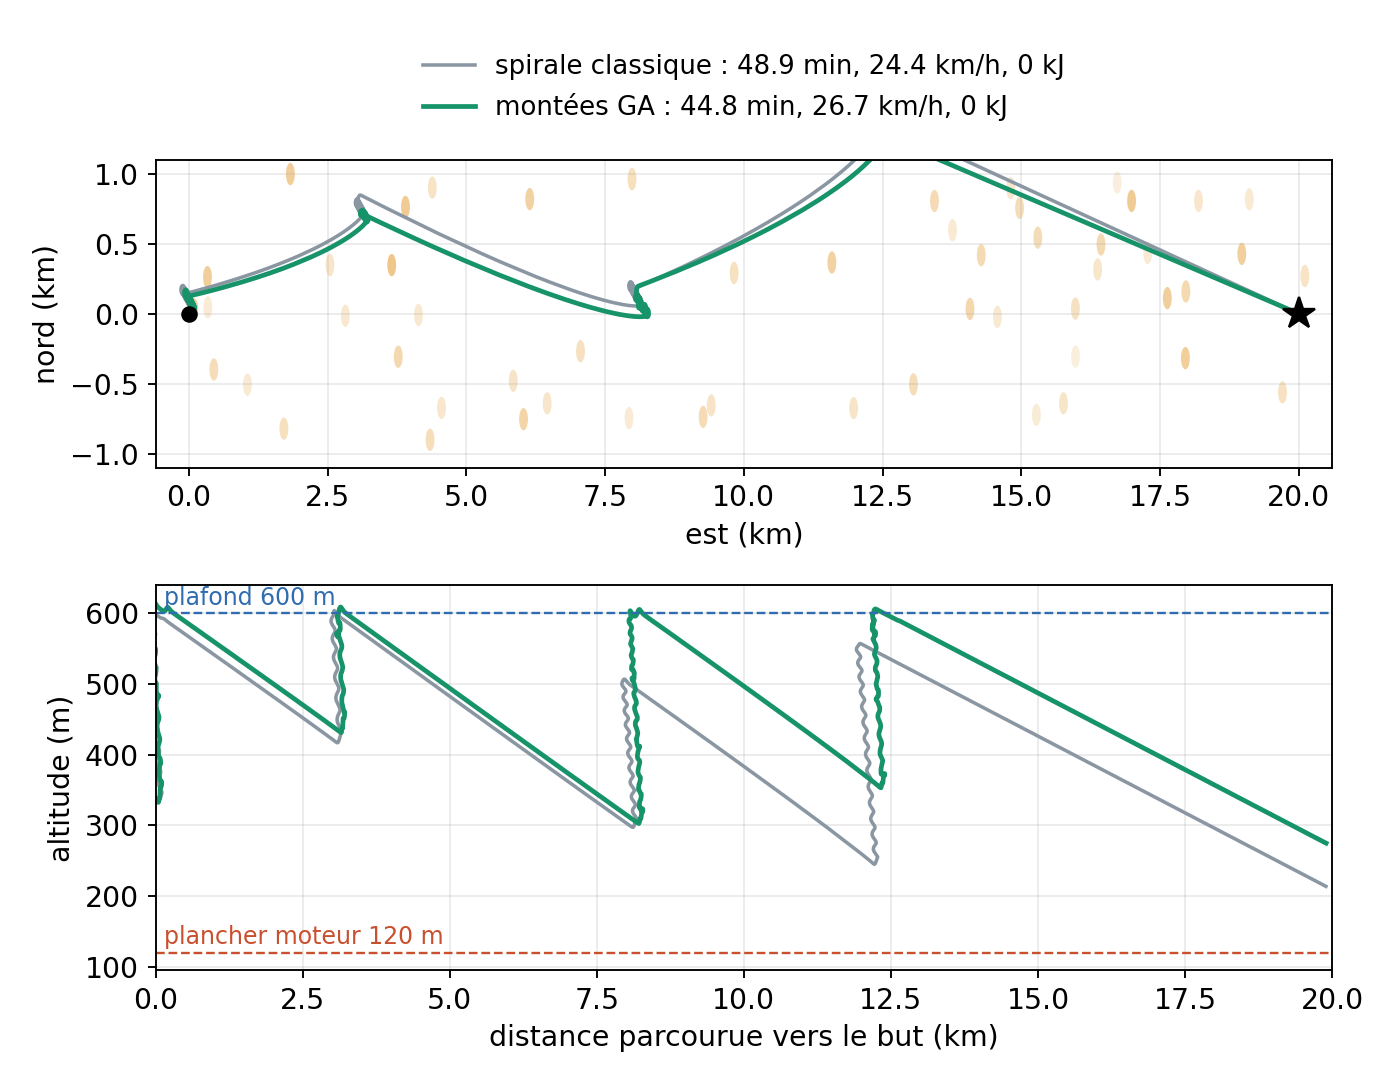
\includegraphics[width=\linewidth]{xc_flight.png}
    \column{0.36\linewidth}
    \small
    \begin{itemize}
      \item Couloir de 2\,km avec $\approx$1 thermique/km² qui dérivent ; départ 250--350\,m, plafond 600\,m, moteur sous 120\,m.
      \item \textbf{Tacticien MacCready} (identique pour tous) : thermique au meilleur rythme de progression, sortie sous le réglage, plané final.
      \item Seule change \textbf{la façon de monter} : spirale classique, ou GA latent par blocs de 60\,s, moteur coupé.
      \item Exemple : même tâche, 4 thermiques chacun ; 48{,}9 contre \good{44{,}8\,min}.
    \end{itemize}
  \end{columns}
\end{frame}

% ---------------------------------------------------------------------------
\begin{frame}{Phase 5 : résultats (Savio, 64 tâches de 20\,km, autopilote protégé)}
  \scriptsize
  \centering
  \begin{tabular}{@{}lccccc@{}}
    \toprule
    Pilote & Batterie & Vitesse & Montée moyenne & Décroche & Sans violation \\ \midrule
    Tout au moteur & 61{,}9\,kJ & 29{,}2\,km/h & -- & 0\,\% & 100\,\% \\
    Spirale classique, MacCready 0{,}5 & 2{,}9\,kJ & 24{,}9\,km/h & 1{,}29\,m/s & 0\,\% & 100\,\% \\
    Spirale classique, MacCready 1 & 19{,}3\,kJ & 28{,}3\,km/h & 1{,}22\,m/s & 0\,\% & 100\,\% \\
    \textbf{Montées GA, MacCready 0{,}5} & 2{,}9\,kJ & \good{28{,}2\,km/h} & \good{2{,}08\,m/s} & \good{0\,\%} & 98\,\% \\
    \textbf{Montées GA, MacCready 1} & \good{4{,}7\,kJ} & \good{29{,}5\,km/h} & \good{2{,}07\,m/s} & \good{0\,\%} & 100\,\% \\
    GA avec marge de 20\,\%, MacCready 1 & 4{,}7\,kJ & 29{,}0\,km/h & 1{,}90\,m/s & 0\,\% & 100\,\% \\
    \bottomrule
  \end{tabular}\par\medskip
  \small
  \begin{itemize}
    \item \good{+61\,\% de vitesse de montée} ; à réglage égal \good{+3{,}3\,km/h} pour la même batterie, plus rapide sur \textbf{89\,\%} des tâches.
    \item À MacCready 1 : \good{la vitesse du vol au moteur avec 13 fois moins de batterie} (meilleur que la spirale sur 73\,\% des tâches).
    \item Sans limiteur, 19 à 69\,\% des vols du GA décrochaient une section. \textbf{Le limiteur d'aile intérieure dans l'autopilote} supprime tous les décrochages \emph{sans} réduire l'avance (2{,}08 contre 2{,}09\,m/s) : le gain ne venait pas du vol au bord du décrochage.
  \end{itemize}
\end{frame}

% ---------------------------------------------------------------------------
\begin{frame}{Phase 6 : distiller la recherche (Savio, 65 situations de test)}
  \begin{columns}[T]
    \column{0.58\linewidth}
    \scriptsize
    \begin{tabular}{@{}lcccc@{}}
      \toprule
      Méthode & Résolues & Coût & Écart & Temps \\ \midrule
      Professeur & 100\,\% & $-4{,}88$ & -- & $\approx$35\,s \\
      64 tirages du prior du VAE & 100\,\% & $-4{,}64$ & $+0{,}24$ & 0{,}24\,s \\
      Générateur distillé, 1 tirage & 94\,\% & $-3{,}52$ & $+1{,}30$ & 0{,}14\,s \\
      \textbf{Générateur distillé, 64 tirages} & 100\,\% & \good{$-5{,}72$} & \good{$-0{,}85$} & \good{0{,}24\,s} \\
      Distillé + GA court (300 vols) & 100\,\% & $-5{,}59$ & $-0{,}71$ & 1{,}4\,s \\
      GA latent (3\,000 vols), la cible & 100\,\% & $-5{,}66$ & $-0{,}78$ & 13{,}4\,s \\
      \bottomrule
    \end{tabular}\par\medskip
    \small Le GA résout 3\,000 situations d'entraînement ; un flow matching conditionnel apprend ses meilleurs points de l'espace latent ; en test, ses tirages sont décodés et volés comme tout candidat.
    \column{0.4\linewidth}
    \small
    \begin{itemize}
      \item \good{Autant que le GA, 57 fois plus vite}, et 0{,}85 de mieux que le professeur dans le temps du prior.
      \item \textbf{Un tirage ne suffit pas} : c'est « proposer 64, vérifier par la physique, garder le meilleur » qui marche.
      \item Une recherche courte par-dessus n'apporte rien.
      \item \textbf{Le plan initial tient}, dans l'ordre découvert : explorer hors ligne (GA dans un espace appris), distiller (flow matching), proposer et vérifier en vol.
    \end{itemize}
  \end{columns}
\end{frame}

% ---------------------------------------------------------------------------
\begin{frame}{Phase 6 : le générateur en vol de 20\,km, et un tour de DAgger}
  \scriptsize
  \centering
  \begin{tabular}{@{}lcccc@{}}
    \toprule
    Montées (64 tâches de 20\,km), MacCready 0{,}5 / 1 & Montée moyenne & Vitesse & Batterie & Temps par plan \\ \midrule
    Spirale classique & 1{,}29 / 1{,}22\,m/s & 24{,}9 / 28{,}3\,km/h & 2{,}9 / 19{,}3\,kJ & réflexe \\
    GA latent & 2{,}08 / 2{,}07\,m/s & 28{,}2 / 29{,}5\,km/h & 2{,}9 / 4{,}7\,kJ & $\approx$13\,s \\
    Générateur distillé sur S1 seulement & \bad{1{,}50 / 1{,}17\,m/s} & 25{,}1 / 28{,}8\,km/h & 4{,}2 / 20{,}2\,kJ & 0{,}24\,s \\
    \textbf{Générateur après un tour de DAgger} & \good{2{,}23 / 2{,}20\,m/s} & \good{28{,}5 / 30{,}2\,km/h} & 2{,}9 / 4{,}7\,kJ & \good{0{,}24\,s} \\
    \bottomrule
  \end{tabular}\par\medskip
  \small
  \begin{itemize}
    \item \textbf{Hors de sa distribution, le premier générateur s'effondre} : appris sur des départs en vol droit entre 180 et 320\,m, il replanifie en plein virage jusqu'à 600\,m, sans connaître l'inclinaison actuelle.
    \item \textbf{DAgger} : 1\,095 plans de montée gagnés par le GA en vol sont enregistrés (situation, état de l'avion, point latent) ; le générateur est réentraîné dessus, avec l'inclinaison, la vitesse et le $C_L$ dans sa condition.
    \item Résultat : \good{aussi bien que le GA, et légèrement mieux} (plus rapide sur 84\,\% et 77\,\% des tâches), en 0{,}24\,s par plan ; à MacCready 1, \good{plus rapide que le moteur} (30{,}2 contre 29{,}2\,km/h) avec 13 fois moins de batterie ; 0 décrochage ; inchangé sur les situations S1 ($-5{,}72$).
  \end{itemize}
\end{frame}

% ---------------------------------------------------------------------------
\begin{frame}{Ce qu'on a découvert}
  \small
  \begin{enumerate}
    \item \textbf{Un GA échoue sur la trajectoire brute mais bat son professeur dans un espace appris.} Même algorithme, autre représentation : 55\,\% $\to$ 100\,\% résolues, puis $-0{,}82$ à $-0{,}84$ sous le professeur.
    \item \textbf{Mettre la physique dans le décodeur} (sortir des commandes bornées et les simuler) règle la faisabilité : 20\,\% $\to$ 100\,\%. 64 tirages égalent le professeur en 0{,}2\,s.
    \item \textbf{Un optimiseur trouve d'abord les défauts du simulateur} (énergie gratuite d'Euler, $\times3$).
    \item \textbf{La limite réelle d'un planeur en spirale est le décrochage de l'aile intérieure}, pas le rayon : le bon remède est une orbite plus rapide, pas plus large ; la marge au décrochage (charge alaire, $C_{L,\max}$) gouverne le gain, la traînée non.
    \item \textbf{Un MPC à énergie terminale procrastine} : un horizon glissant de 60\,s repousse sans fin le gain ; il faut viser la fin du vol (horizon qui rétrécit).
    \item \textbf{En vol, savoir où est le thermique compte plus que bien planifier} : 15\,m d'erreur coûtent plus que la turbulence.
    \item \textbf{Sur 20\,km, mieux spiraler vaut des km/h} ($+3{,}3$) ou une batterie divisée par 13 ; \textbf{la sécurité se met dans l'autopilote}, pas dans les marges du plan.
    \item \textbf{La recherche se distille, à condition de lui montrer les situations du vol} : un flow matching entraîné sur les solutions du GA fait aussi bien que lui en 0{,}24\,s, mais seulement après un tour de DAgger sur les états rencontrés en vol.
  \end{enumerate}
\end{frame}

% ---------------------------------------------------------------------------
\begin{frame}{Portée et limites}
  \begin{columns}[T]
    \column{0.5\linewidth}
    \textbf{Ce que les résultats couvrent}
    \small
    \begin{itemize}
      \item Un motoplaneur de 4{,}2\,kg (SB-XC), polaire estimée testée à $\pm20$\,\%.
      \item Thermiques isolés, champs de thermiques sur 20\,km, vent 0--4\,m/s, turbulence légère.
      \item Tests sur situations jamais vues ; 64 à 80 situations par comparaison ; comparaisons appariées.
    \end{itemize}
    \column{0.5\linewidth}
    \textbf{Ce qu'ils ne couvrent pas encore}
    \small
    \begin{itemize}
      \item \bad{Simulation seulement} : point-masse 3 DDL + aile par tronçons, pas de 6 DDL ni de vol réel.
      \item Modèle de thermique synthétique (Allen + cœur gaussien) ; en phase 5, \bad{thermiques connus exactement}.
      \item 17\,\% des situations restent non résolues par le professeur et sont exclues des tests.
      \item Le générateur (0{,}24\,s par plan sur un cœur de serveur) n'est pas encore mesuré sur calculateur embarqué ; un seul tour de DAgger, un seul run par configuration.
      \item Au-dessus de 320\,m, le VAE sort de ses données d'entraînement.
    \end{itemize}
  \end{columns}
\end{frame}

% ---------------------------------------------------------------------------
\begin{frame}{Moyens de calcul}
  \small
  \begin{itemize}
    \item \textbf{Savio (UC Berkeley, compte ic\_piml)} : tableaux SLURM de 21 n\oe uds de 32 c\oe urs pour le professeur (15\,080 situations en $\approx$15\,min), GPU A40 pour les élèves, un n\oe ud par étude (sensibilité, boucle fermée, 20\,km).
    \item \textbf{PC de calcul (qltus1, qltus2)} : 3\,080 situations en 1\,h\,15 ; Python 3.14 environ 4 fois plus rapide par c\oe ur que le gros PC.
    \item \textbf{Code} : NumPy/SciPy pour l'optimisation et la simulation, PyTorch pour les élèves ; 69 tests ; dépôt public \texttt{github.com/clementdumeril/GeneticWing}.
    \item \textbf{Visualiseurs 3D} : vols de 60\,s autour d'un thermique, et vol de 20\,km (pages autonomes dans \texttt{docs/viewer}).
  \end{itemize}
\end{frame}

% ---------------------------------------------------------------------------
\begin{frame}{La suite}
  \begin{enumerate}
    \item \textbf{Recentrer le thermique en vol} (estimateur à partir du vario, comme ArduPilot) : c'est la plus grosse perte mesurée (de $-5$ à $-2$), et la phase 5 suppose aujourd'hui des thermiques connus.
    \item \textbf{Réentraîner le VAE sur des montées jusqu'à 600\,m}, et le conditionner sur la charge alaire et $C_{L,\max}$.
    \item \textbf{Les 17\,\% de situations non résolues} par le professeur.
    \item \textbf{Un second tour de DAgger} (les montées du générateur lui-même, relabellisées par le GA), puis le générateur dans la boucle fermée de la phase 4 (rafales, croyance fausse).
    \item \textbf{Vers le réel} : simulateur 6 DDL ou SITL, puis mesures de l'avion.
  \end{enumerate}
\end{frame}

\end{document}
